%%%%%%%%%%%%%%%%%%%%%%%%%%%%%%%%%%%%%%%%%%%%%%%%%%%%%%%%%%%%%%%%%%%%%%%%%%%%%%%%%%%%%%%%%%%%%%%
%Plantilla: para la realizaci�n de informes.
%Curso:     Simulaci�n estad�stica.
%Profesor:  Johann A. Ospina.
%%%%%%%%%%%%%%%%%%%%%%%%%%%%%%%%%%%%%%%%%%%%%%%%%%%%%%%%%%%%%%%%%%%%%%%%%%%%%%%%%%%%%%%%%%%%%%%


%Establece el tipo de documento (art�culo), tama�o de letra (10pt) a una columna.
\documentclass[letterpaper,12pt,onecolumn,titlepage]{article} 
 
 
% Cargar paquetes
\usepackage{verbatim}
\usepackage{mathrsfs}
\usepackage{amsmath}
\usepackage{amssymb}
\usepackage{subfigure}
\usepackage{ucs}
\usepackage[latin1]{inputenc}
\usepackage[spanish]{babel}
\usepackage{fontenc}
\usepackage{graphicx}
\usepackage{anysize}
\usepackage{fancyhdr}
\usepackage[comma,authoryear]{natbib}
\usepackage{url} %paquete para definir url
\usepackage{hyperref}  %hipervinculos

%Estilo de la p�gina
\pagestyle{fancy}

%Establecer el margen
\marginsize{2cm}{2cm}{1cm}{1cm}
\setlength{\headheight}{13.1pt}


% Portada
\title{
    \textbf{Laboratorio N.4}\
    ~\\{Introduccion a Los Metodos Estadisticos}   
    ~\\{Prueba de Hipotesis y Regresion}}
\author{
    {Diana Carolina Arias Sinisterra Cod. 1528008}
 ~\\{Kevin Steven Garcia Chica Cod. 1533173}
 ~\\{Cesar Andres Saavedra Vanegas Cod. 1628466}}

\date{
     \textbf{Universidad Del Valle}\   
    ~\\{Facultad De Ingenieria}
    ~\\{Estadistica}
    ~\\{Diciembre}
    ~\\{2017}}
 
 
 
\decimalpoint %Poner punto decimal
 
\begin{document}
 
% Se aplica el formato a las p�ginas. Se despliegan: portada e �ndices de materias, figuras y tablas
\renewcommand{\listtablename}{}
\renewcommand{\tablename}{Tabla}
\maketitle
\setcounter{page}{2}
\tableofcontents{}
%\thispagestyle{empty}
%\newpage
\listoffigures{}
\listoftables{}

\thispagestyle{empty}

\newpage
\fancyhead{}
\fancyfoot{}
 
% Encabezado y pie de pagina
\lhead{Introduccion a los Metodos Estadisticos}
\lfoot{Universidad Del Valle}
\rfoot{\thepage}

% Estilo de la bibliograf�a
\bibliographystyle{apalike}
 
% Desarrollo de los contenidos del documento
\section{Prueba De Hipotesis}
\subsection{Situaci\'{o}n 1}

\pagebreak \subsection{Situaci\'{o}n 2}
\subsection{Punto A.}
\subsection{Punto B.} 

\pagebreak\subsection{Situaci\'{o}n 3}
\subsection{Punto A.}
\subsection{Punto B.} 

\pagebreak\subsection{Situaci\'{o}n 4}

\pagebreak\subsection{Situaci\'{o}n 5}
\subsection{Punto A.}
\subsection{Punto B.} 
\subsection{Punto C.}

\pagebreak\subsection{Situaci\'{o}n 6}
\subsection{Punto C.}
\subsection{Punto D.} 

\pagebreak\subsection{Situaci\'{o}n 7}
\subsection{Punto A.}
\subsection{Punto B.}

\pagebreak\section{Regresion}
\subsection{Situaci\'{o}n 1}
\subsection{Punto A.}
\begin{itemize}
\item Reducci\'{o}n porcentual del total de s\'{o}lidos: El total de s\'{o}lidos disueltos (a menudo abreviado como TDS, del ingl\'{e}s: Total Dissolved Solids) es una medida del contenido combinado de todas las sustancias inorg\'{a}nicas y org\'{a}nicas contenidas en un l\'{i}quido en forma molecular, ionizada o en forma de suspensi\'{o}n micro-granular (sol coloide). 
Los TDS (Total dissolved solids) son la suma de los minerales, sales, metales, cati\'{o}nes o aniones disueltos en el agua. Esto incluye cualquier elemento presente en el agua que no sea (H20) mol\'{e}cula de agua pura y s\'{o}lidos en suspensi\'{o}n. (S\'{o}lidos en suspensi\'{o}n son part\'{i}culas \'{o} sustancias que ni se disuelven ni se asientan en el agua, tales como pulpa de madera.)
En general, la concentraci\'{o}n de s\'{o}lidos disueltos totales es la suma de los cati\'{o}nes (carga positiva) y aniones (cargado negativamente) iones en el agua.
\item Reducci\'{o}n porcentual de demanda bioqu\'{i}mica de oxigeno: La demanda bioqu\'{i}mica de ox\'{i}geno (DBO) es un par\'{a}metro que mide la cantidad de diox\'{i}geno consumido al degradar la materia org\'{a}nica de una muestra l\'{i}quida.
\end{itemize} 
\pagebreak\subsection{Punto B.}
~\\ \begin{figure}[!h]
    \begin{center}
        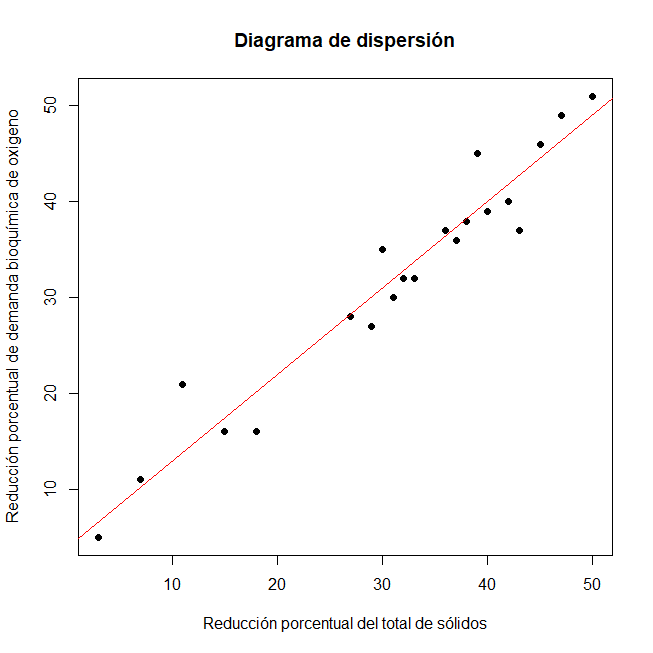
\includegraphics[width=10cm]{Figuras/punto1b.png}
        \caption{Gr\'{a}fica de dispersi\'{o}n con recta de ajuste entre las variables X y Y}
        \label{fig:Densidad}
    \end{center}
\end{figure}
~\\ En esta imagen podemos ver que hay una correlaci\'{o}n positiva bastante fuerte, por lo que esperamos que el coeficiente de correlaci\'{o}n sea cercano a 1. Tambi\'{e}n podemos ver que las distancias de los datos o los puntos a la recta de ajuste son considerablemente peque\~{n}as, por lo cu\'{a}l creemos que el $R^2$ es tambi\'{e}n cercano a 1, dici\'{e}ndonos esto, que el modelo ajustado representara en un alto porcentaje la variaci\'{o}n total de Y.
~\\ Procedemos a calcular los dos valores mencionados:
\begin{itemize}
\item Coeficiente de correlaci\'{o}n: $\hat{\rho}=r=\frac{\sum\limits_{i=1}^{n}(x_{i}-\bar{x})(y_{i}-\bar{y})}{\sqrt{\sum\limits_{i=1}^{n}(x_{i}-\bar{x})^2}\cdot\sqrt{\sum\limits_{i=1}^{n}(y_{i}-\bar{y})^2}}$
~\\ $\bar{x}=31.095238$ y $\bar{y}=31.9523809$, entonces:
~\\ $$\hat{\rho}=r=\frac{3202.095238}{\sqrt{3543.809524\cdot\sqrt{3086.952381}}}=\frac{3202.095238}{3307.502267}=0.9681$$
\item Coeficiente de determinaci\'{o}n $R^2$: $R^2=r^2=0.9372$
~\\ Tal y como esper\'{a}bamos, el coeficiente de correlaci\'{o}n lineal, nos arrojo un resultado de 0.9681 que es bastante alto. Este resultado nos dice que a medida que X aumenta, Y tambi\'{e}n aumenta en una proporci\'{o}n aproximada de 0.9681. Con respecto al $R^2$, tambi\'{e}n nos arroj\'{o} un valor que esper\'{a}bamos (0.9372) que es bastante alto; este valor nos dice que el $93.72\%$ de la variabilidad total de la variable Y, es explicada por la variable X.
Entonces, seg\'{u}n lo anterior, concluimos que estas dos variables tienen una relaci\'{o}n positiva demasiado fuerte, es decir, cuando aumenta X, Y tambi\'{e}n aumentara, y por el $R^2$ concluimos que X es una buena variable explicativa para Y.
\end{itemize} 
\subsection{Punto C.}
~\\ Para evaluar la asociaci\'{o}n lineal entre las variables X y Y, tendremos que plantear las hip\'{o}tesis sobre $\rho$ de la siguiente manera:

~\\ $H_{0}$: $\rho=0$ (No hay correlaci\'{o}n lineal)
~\\ $H_{1}$: $\rho\neq 0$ (Hay correlaci\'{o}n lineal)

~\\ $T_{\rho}=\frac{r-\rho}{\sqrt{\frac{1-r^2}{n-2}}}$
~\\ Reemplazando los valores, teniendo en cuenta que por el punto anterior $r=0.9681$, tenemos:
~\\ $T_{\rho}=\frac{0.9681}{\sqrt{\frac{1-(0.9681)^2}{21-2}}}=16.84139$

~\\ Tomando $\alpha=0.05$, $T_{(0.975;19)}=2.093$
~\\ Como $T_{\rho}=16.84139>2.093$, rechazamos $H_{0}$ y concluimos que con una confianza del $95\%$, si existe correlaci\'{o}n lineal entre las dos variables.  
\subsection{Punto D.}
~\\ El modelo ajustado es de la forma: $Y_{i}=\beta_{0}+\beta_{1}X_{i}+e_{i}$
~\\ $$\hat{\beta_{1}}=\frac{\sum\limits_{i=1}^{n}x_{i}y_{i}-n\bar{x}\bar{y}}{\sum\limits_{i=1}^{n}{x_{i}}^2 - n\bar{x}^2}=\frac{24067-21(31.095238)(31.9523809)}{23849-21(31.095238)^2}=\frac{3202.095336}{3543.809648}=0.903574$$

~\\ $$\hat{\beta_{0}}=\bar{y}-\hat{\beta_{1}}\bar{x}=31.9523809-(0.903574\cdot 31.095238)=3.855532$$

~\\ El modelo ajustado queda: $Y_{i}=3.855532+0.903574 X_{i}+ e_{i}$

~\\ \textbf{INTERPRETACI\'{O}N:}
~\\ $\hat{\beta_{0}}=3.855532$ : Sin tener en cuenta la variabilidad de la reducci\'{o}n porcentual del total de s\'{o}lidos, se espera una reducci\'{o}n porcentual de demanda bioqu\'{i}mica de oxigeno de 3.855532.

~\\ $\hat{\beta_{1}}=0.903574$ : Por cada unidad adicional de la reducci\'{o}n porcentual del total de s\'{o}lidos, se espera que la reducci\'{o}n porcentual de demanda bioqu\'{i}mica de oxigeno aumente en promedio en 0.903574 unidades.

\pagebreak\subsection{Punto E.}
~\\ Los indicadores utilizados para evaluar la bondad de ajuste de un modelo son el $\rho$ y el $R^2$, como ya los obtuvimos en el punto b, vamos a interpretarlos.

~\\ $\rho=0.9681$: Este valor nos indica que existe una correlaci\'{o}n positiva bastante fuerte (casi perfecta), es decir, cuando x aumenta, y aumenta casi en la misma proporci\'{o}n. Cuando tenemos una correlaci\'{o}n tan alta entre las dos variables, podemos estar seguros de que el modelo ajustado ser\'{a} un buen modelo ($R^2$ tendiendo a 1) para explicar Y en t\'{e}rminos de X.

~\\ $R^2=0.9372$: Este valor nos dice que el $93.72\%$ de la variabilidad total de variable Y(reducci\'{o}n porcentual de demanda bioqu\'{i}mica de oxigeno) es exlicada por la variable X(reducci\'{o}n porcentual del total de s\'{o}lidos). Lo que en el fondo nos dice que el modelo es bastante bueno, ya que las distancias de los datos o los puntos a la recta de regresi\'{o}n ajustada, son muy peque\~{n}as.

\subsection{Punto F.}
~\\ \textbf{Para $\beta_{0}$:} $\langle \beta_{0} \rangle_{(1-\alpha)\%}=\langle \hat{\beta_{0}}\pm t_{(\frac{\alpha}{2},n-2)}\sqrt{V(\hat{\beta_{0}})} \rangle$

~\\ $V(\hat{\beta_{0}})=\frac{\hat{\sigma^2} \sum\limits_{i=1}^{n}{x_{i}}^2}{n S_{xx}}$

~\\ $\hat{\sigma^2}=\frac{1}{n-2}[S_{yy}-\hat{\beta_{1}}S_{xy}]=\frac{1}{21-2}[3086.952381-(0.903574\cdot 3202.095238)]=\frac{1}{19}(193.6223784)=10.1906515$

~\\ Entonces, reemplazando: $V(\hat{\beta_{0}})=\frac{10.196515\cdot 23849}{21\cdot 3543.809524}=3.265746$

~\\ Ahora, con $\alpha=0.05$:
~\\ $$\langle \beta_{0} \rangle_{0.95\%}=\langle 3.855532 \pm 2.093\cdot \sqrt{3.265746} \rangle$$
~\\ $$(0.073193 ; 7.6378708) $$

~\\ \textbf{Para $\beta_{1}$:} $\langle \beta_{1} \rangle_{(1-\alpha)\%}=\langle \hat{\beta_{1}}\pm t_{(\frac{\alpha}{2},n-2)}\sqrt{V(\hat{\beta_{0}})} \rangle$

~\\ $V(\hat{\beta_{1}})=\frac{\hat{\sigma^2}}{S_{xx}}$
~\\ Ya sabemos que $\hat{\sigma^2}=10.1906515$

~\\ Entonces: $V(\hat{\beta_{1}})=\frac{10.1906515}{3543.809524}=0.00287562$

~\\ Ahora, con $\alpha=0.05$:
~\\ $$\langle \beta_{1} \rangle_{0.95\%}=\langle 0.903574 \pm 2.093\cdot \sqrt{0.00287562} \rangle$$
~\\ $$(0.791337 ; 1.0158107) $$
\subsection{Punto G.}
~\\ \textbf{ESTIMACI\'{O}N PUNTUAL:}
~\\ $E[Y|X]=E[\beta_{0}+\beta_{1}x1+e]=E[\beta_{0}]+E[\beta_{1}x_{1}]+E[e]$, sabemos que $E[e]=0$, por los supuestos del modelo lineal.
~\\ Entonces: $\hat{E[Y|X]}=\hat{\beta_{0}}+\hat{\beta_{1}}x_{1}$
~\\ Por consiguiente: $E[Y|X=30]=\hat{\beta_{0}}+\hat{\beta_{1}}\cdot 30=3.855532+0.903574(30)=30.962752$

~\\ El valor esperado de la reducci\'{o}n de la demanda bioqu\'{i}mica de oxigeno cuando se reduce a $30\%$ el porcentaje total de s\'{o}lidos es de $30.962752\%$.


~\\ \textbf{ESTIMACI\'{O}N POR INTERVALOS:}
~\\ No tenemos formula para la estimaci\'{o}n or intervalos de la esperanza de Y dado un valor $X=x_{0}$, esto es $E[Y|X=x_{0}]$ por lo cual, trataremos de construirlo, como un intervalo para la media, esto seria:
~\\ $\langle E[Y|X=x_{0}] \rangle_{1-\alpha\%}=\langle \hat{E[Y|X=x_{0}]} \pm t_{(\frac{\alpha}{2};n-2)}\cdot \sqrt{V(\hat{E[Y|X=x_{0}]})}\rangle $

~\\ Debemos hallar $V(\hat{E[Y|X=x_{0}]})$, ya que no la conocemos.

~\\ Sabemos que: $\hat{E[Y|X=x_{0}]}=\hat{\beta_{0}}+\hat{\beta_{1}}x_{0}$  , como $\hat{\beta_{0}}=\bar{Y}-\hat{\beta_{1}}\bar{X}$ 
~\\ $$\hat{E[Y|X=x_{0}]}=\bar{Y}-\beta_{1}\bar{X}+\hat{\beta_{1}}x_{0}$$
~\\ $$\hat{E[Y|X=x_{0}]}=\bar{Y}+\hat{\beta_{1}}(x_{0}-\bar{X})$$

~\\ Ahora, procedemos a calcular lo que nos interesa:
~\\ $$Var(\hat{E[Y|X=x_{0}]})=Var(\bar{Y})+Var[\hat{\beta_{1}}(x_{0}-\bar{X})]$$
~\\ $$=Var(\bar{Y})+(x_{0}-\bar{X})^2 Var(\hat{\beta_{1}})$$ 
~\\ como $V(\hat{\beta_{1}})=\frac{\hat{\sigma}^2}{S_{xx}}$ y $V(\bar{Y})=\frac{1}{n}\hat{\sigma}^2$, reemplazando nos queda:
~\\ $$Var(\hat{E[Y|X=x_{0}]})=\frac{1}{n}\hat{\sigma}^2 + (x_{0}-\bar{X})^2 \cdot \frac{\hat{\sigma}^2}{S_{xx}}$$
~\\ $$=\hat{\sigma}^2 \left( \frac{1}{n}+\frac{(x_{0}-\bar{X})^2}{S_{xx}}\right)$$

~\\ Entonces, nuestro intervalo de confianza construido para el valor esperado de Y dado un valor $X=x_{0}$ quedara:
~\\ $\langle E[Y|X=x_{0}] \rangle _{(1-\alpha)\%}=\langle \hat{E[Y|X=x_{0}]}\pm t_{(\frac{\alpha}{2};n-2)}\sqrt{(\frac{1}{n}+\frac{(x_{0}-\bar{X})^2}{S_{xx}})\cdot \hat{\sigma^2}} \rangle$

~\\ Ahora, volviendo a nuestro problema, tenemos los siguientes datos: $\hat{E[Y|X=30]}=30.962752$, $\hat{\sigma^2}=10.1906515$, $t_{(\frac{\alpha}{2},19)}=2.093$, $\bar{X}=31.095238$ y $S_{xx}=3543.809524$
~\\ Reemplazando en nuestro intervalo, nos queda: 
~\\ $\langle E[Y|X=30] \rangle _{95\%}=\langle 30.962752 \pm 2.093\sqrt{(\frac{1}{21}+\frac{(30-31.095238)^2}{3543.809524})\cdot 10.1906515} \rangle$
~\\ $$=\langle 30.962752 \pm 2.093(0.694132321)\rangle$$
~\\ $$=(29.5099 ; 32.4155)$$
\pagebreak\subsection{Situaci\'{o}n 2}
\subsection{Punto A.}
~\\ \begin{figure}[!h]
    \begin{center}
        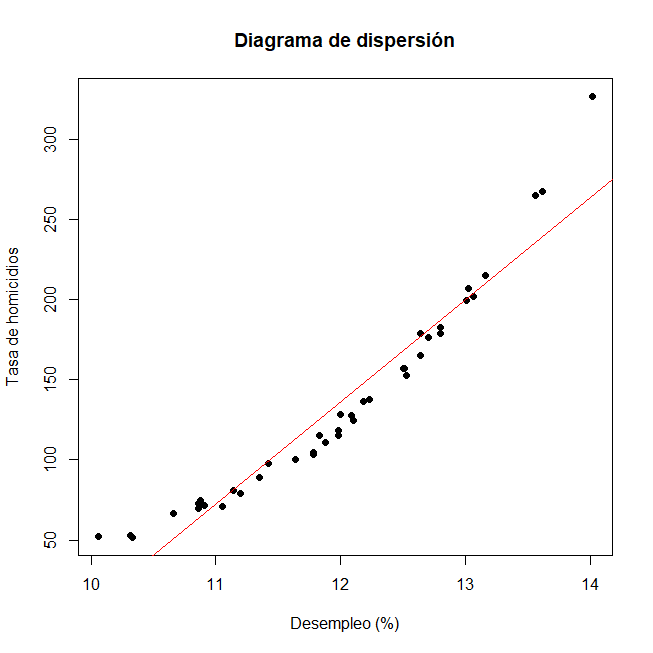
\includegraphics[width=10cm]{Figuras/punto2a.png}
        \caption{Gr\'{a}fica de dispersi\'{o}n con recta de ajuste entre las variables X(desempleo) y Y(Tasa de homicidios)}
        \label{fig:Densidad}
    \end{center}
\end{figure}
~\\ En la imagen anterior, observamos que entre el desempleo(variable X) y la tasa de homicidios(variable Y), existe una correlaci\'{o}n positiva bastante alta (por la forma de la distribuci\'{o}n de los puntos), es decir, a valores altos de X, le corresponden valores altos de Y. Tambi\'{e}n, si observamos la recta de regresi\'{o}n o de ajuste, podemos ver que las distancias en general de cada punto a la recta no son muy amplias, por lo que creemos que el coeficiente de determinaci\'{o}n $R^2$ tambi\'{e}n sera bastante alto (cercano a 1).
~\\ Para corroborar las hip\'{o}tesis que tenemos del punto anterior, hallaremos el indice de correlaci\'{o}n $\rho$ y el coeficiente de determinaci\'{o}n $R^2$.
~\\ Procedemos a calcular los dos valores mencionados:
\begin{itemize}
\item Coeficiente de correlaci\'{o}n: $\hat{\rho}=r=\frac{\sum\limits_{i=1}^{n}(x_{i}-\bar{x})(y_{i}-\bar{y})}{\sqrt{\sum\limits_{i=1}^{n}(x_{i}-\bar{x})^2}\cdot\sqrt{\sum\limits_{i=1}^{n}(y_{i}-\bar{y})^2}}$
~\\ $\bar{x}=11.977$ y $\bar{y}=134.61325$, entonces:
~\\ $$\hat{\rho}=r=\frac{2336.75449}{\sqrt{36.65424\cdot\sqrt{161368.7339}}}=\frac{2336.75449}{2432.046114}=0.9608$$
\item Coeficiente de determinaci\'{o}n $R^2$: $R^2=r^2=0.92317$
\end{itemize}
~\\ Podemos ver con los valores obtenidos que nuestras hip\'{o}tesis son ciertas. El coeficiente de correlaci\'{o}n nos arrojo un resultado de 0.9608, es decir, que existe una correlaci\'{o}n positiva bastante fuerte (casi perfecta), esto es, cuando la variable x aumenta en una unidad, la variable y aumenta casi que en la misma proporci\'{o}n. El coeficiente de determinaci\'{o}n nos arrojo un resultado bastante alto tambi\'{e}n, de 0.92317, esto quiere decir que el modelo que ajustemos posteriormente con dicha variable x(desempleo), explicara el $92.317\%$ de la variaci\'{o}n total de y(tasa de homicidios).

~\\ Procederemos a ajustar el modelo:
~\\ El modelo ajustado es de la forma: $Y_{i}=\beta_{0}+\beta_{1}X_{i}+e_{i}$
~\\ $$\hat{\beta_{1}}=\frac{\sum\limits_{i=1}^{n}x_{i}y_{i}-n\bar{x}\bar{y}}{\sum\limits_{i=1}^{n}{x_{i}}^2 - n\bar{x}^2}=\frac{66827.2703-40(11.977)(134.61325)}{5774.5954-40(11.977)^2}=\frac{2336.75449}{36.65424}=63.7512738$$

~\\ $$\hat{\beta_{0}}=\bar{y}-\hat{\beta_{1}}\bar{x}=134.61325-(11.977\cdot 63.7515738)=-628.935756$$

~\\ El modelo ajustado queda: $Y_{i}=-628.935756+63.7512738X_{i}+ e_{i}$
\subsection{Punto B.}
~\\ Para estimar la tasa de homicidios cuando disminuya la tasa de desempleo al $11\%$, debemos hallar o estimar el valor esperado de Y dado que X tome el valor de 11, esto es, $\hat{E[Y|X=11]}$:
~\\ $\hat{E[Y|X=11]}=-628.9357563+63.7512738(11)=72.3282555$
~\\ En conclusi\'{o}n, la tasa de homicidios cuando el desempleo sea del $11\%$ es de aproximadamente 72.3282 casos por 100.000 habitantes. 
\subsection{Punto C.}
~\\ Para la realizaci\'{o}n del informe con las conclusiones mas importantes, debemos tener en cuenta la interpretaci\'{o}n de los valores encontrados en el literal a.
\begin{itemize}
\item $\hat{\beta_{0}}=-628.9357563$: Sin tener en cuenta la variaci\'{o}n la tasa de desempleo, se espera una tasa de homicidios de $-628.9357563$ casos por cada $100.000$ habitantes, obviamente esta variable no toma valores negativos, entonces decimos que cuando el desempleo es 0, el numero de homicidios tambien sera 0.
\item $\hat{\beta_{1}}=63.7512738$: Cuando la tasa de desempleo aumente en una unidad (en $1\%$) la tasa de homicidios aumentara 63.7512 casos por cada $100.000$ habitantes. En la interpretaci\'{o}n de este coeficiente podemos ver la importancia del desempleo en la tasa de homicidios, ya que, con tan solo una unidad de aumento en el desempleo, la tasa de homicidios aumenta demasiado.
\item Con respecto a la correlaci\'{o}n entre estas dos variable, vemos que tienen una correlaci\'{o}n lineal casi perfecta ($\rho=0.9608$), esto nos dice que cuando X(tasa de desempleo) aumenta, la variable Y(Tasa de homicidios) tambien aumenta. Y, el coeficiente de determinaci\'{o}n $R^2$, que nos arrojo un resultado de 0.92317, nos dice que el $92.317\%$ de la variaci\'{o}n total de la variable Y(Tasa de homicidios), es explicada por la tasa de desempleo (variable X). Entonces concluimos que esta variable (Desempleo) es muy influyente e importante en la tasa de homicidios.
\item Conclusi\'{o}n: Seg\'{u}n todo lo anterior, podr\'{i}amos concluir que para disminuir un poco la problem\'{a}tica de la tasa de homicidios en la comunidad estudiada, se deben enfocar en disminuir primero la tasa de desempleo, ya que una conlleva a la otra (una disminuci\'{o}n en la tasa de desempleo causa una disminuci\'{o}n considerable en la tasa de homicidios). Entonces una posible soluci\'{o}n indirecta a la tasa de homicidios, es por ejemplo, aumentar el numero de empleos.
\end{itemize}
\bibliography{Bibliografia}
\end{document}








